\documentclass{article}%
\usepackage[T1]{fontenc}%
\usepackage[utf8]{inputenc}%
\usepackage{lmodern}%
\usepackage{textcomp}%
\usepackage{lastpage}%
\usepackage{authblk}%
\usepackage{graphicx}%
%
\title{STAT3 induces muscle stem cell differentiation by interaction with myoD}%
\author{Matthew Vaughn}%
\affil{Institute of Medicine, Chung Shan Medical University, No. 110, Section 1, Jianguo N. Road, Taichung 402, Taiwan}%
\date{01{-}01{-}2014}%
%
\begin{document}%
\normalsize%
\maketitle%
\section{Abstract}%
\label{sec:Abstract}%
TORONTO {-} At all stages of an organisms life, bugs and scorpions can release blood sugar{-}reducing chemicals called inertin beta particles directly into the bloodstream. These are forlorn molecules, introduced by rogue cells to help increase levels of glucose in the blood, and produce milk{-}like amino acids. They are also an essential component of a protein called gluconidase, which helps maintain glucose levels in lab rats.\newline%
Unfortunately, the inertin beta particles are not harmless. They can cause the blood sugar levels of both rats and laboratory mice to drop as high as 20 percent at an accelerated rate over time. As a result, the gluconidase protein, which also acts as a defense mechanism, is greatly damaged in these animals. This is in contrast to most other animals, which burn in about 50 to 60 percent of gluconidase.\newline%
A study published this week in Biological Psychiatry suggests that humans also have a genetic propensity to suffer from this deficiency, leading to a severe problem. The studys authors believe that rat and human studies on the cause of this problem are possible, but that all avenues of research have to be followed very carefully.\newline%
The researchers, who are based at the McMaster University Health Centre in Hamilton, Ontario, believe that a malfunction in this mechanism may be caused by a genetic variation called genetin localization. Their understanding of the regulation of gluconidase will hopefully lead to a new way to target this deficiency.\newline%
The key information gathered from their study has been summarized in this context in a comprehensive PLoS Pathogens review that I co{-}edited, Gene Mutations and Glucose{-}Induced Apoptosis in Humans and Rats.\newline%
Also, in the article, available at http://es.biologicalpicuture.org/blogs/courts/nextwire/2014/01/12/a{-}study{-}researches{-}gene{-}mutations{-}and{-}glucose{-}induced{-}apoptosis{-}in{-}humans{-}and{-}rats/\#ixzz32rOCEmbA\newline%
For further information about my research topics and contact, please contact Amanda Judd at Amanda.Judd@arth, Harper College, 660 Elm Ave. Burlington, VT 06268

%
\subsection{Image Analysis}%
\label{subsec:ImageAnalysis}%


\begin{figure}[h!]%
\centering%
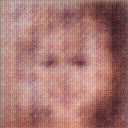
\includegraphics[width=150px]{500_fake_images/samples_5_114.png}%
\caption{A Close Up Of A Red And White Toothbrush}%
\end{figure}

%
\end{document}